\chapter[PPM Generation and Demodulation]{PPM Generation and Demodulation}

\section*{Aim}

To set-up and implement circuit to carry out pulse position modulation. To design demodulating circuit to detect the message from pulse position modulated wave.
\section*{Theory}
In pulse position modulation method, the position of a narrow pulse is varied within the period of the carrier in accordance with the amplitude of analog modulating signal as shown. Before and after modulation, the amplitude and frequency of the carrier remain constant. Only the pulse position is varying.

Waveforms showing pulse carriers whose position is modulated by message is shown in Figure \ref{ppmckt}.

Modulation can be carried out using a 555 timer IC configured in monostable multivibrator mode. The width of the pulse is set to be very narrow(10\% duty cycle) by the time constant of the circuit. The monostable multivibrator is triggered by  the output of a PWM signal (See the waveform).  The result is PPM modulation.

The demodulation of PPM waveform can be done by regenerating PWM waveform using 555 timer IC as a switch. A lowpass filter which passes message signal frequenies but blocks the carrier signal is used then to demodulate the message signal.

%\begin{figure}[h]
%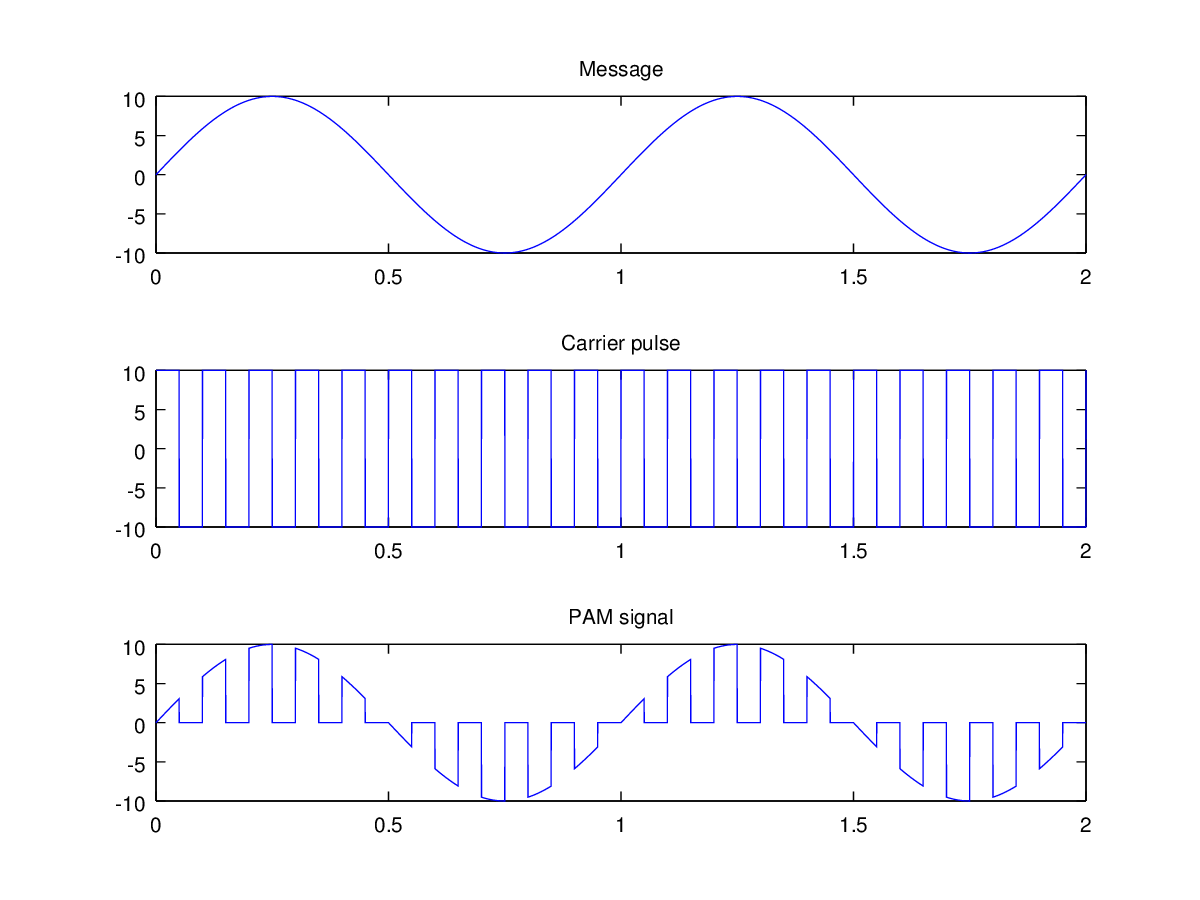
\includegraphics[width=\textwidth]{pam1.png}
%\caption{PAM modulation using transistor}
%\label{PAMmod1}
%\end{figure}
%
%\begin{figure}[h]
%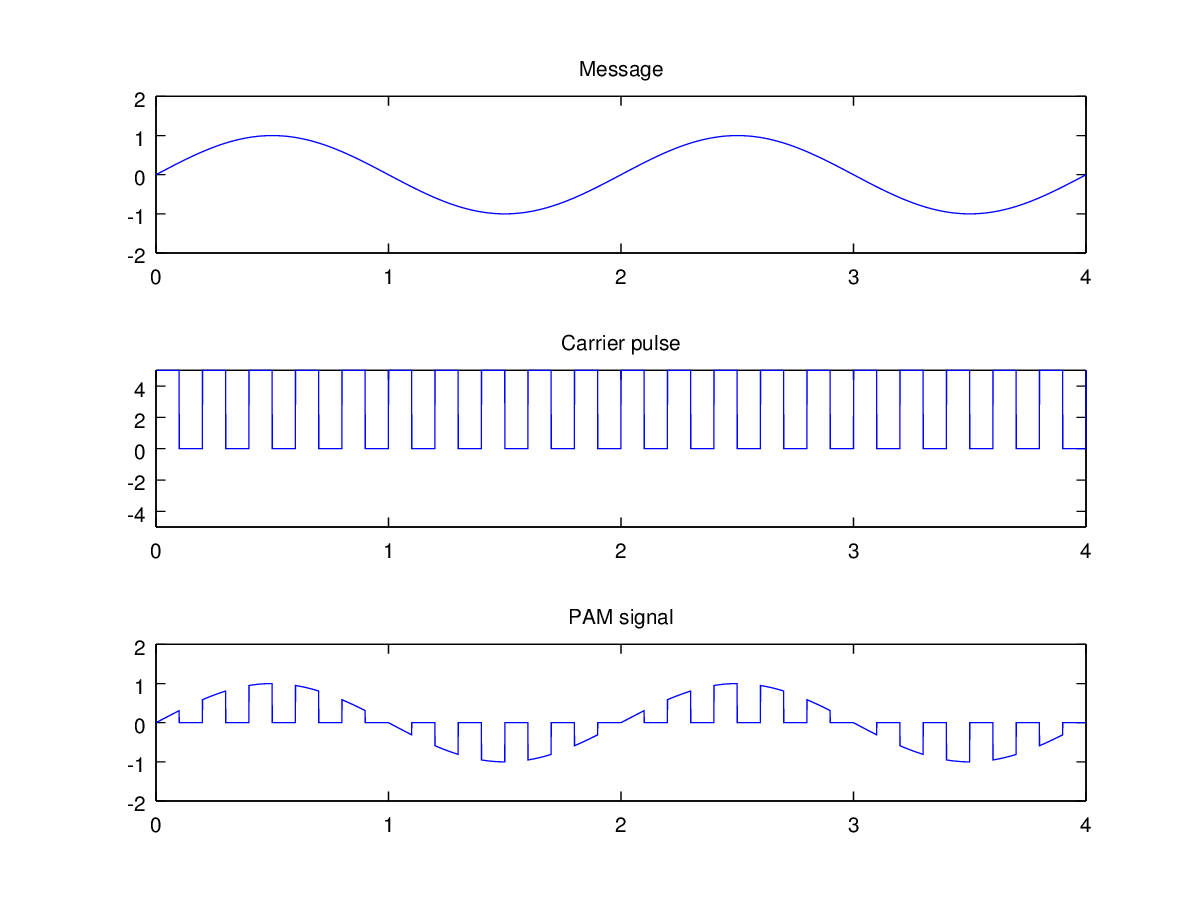
\includegraphics[width=\textwidth]{pam2.png}
%\caption{PAM modulation using switching IC}
%\label{PAMmod2}
%\end{figure}

\section*{Design}
\subsection*{Modulation}

One technique to implement PPM is to use 555 timer IC in monostable multivibrator mode. Let the carrier frequency be 5 kHz. Then $T= 0.2 ms$. The pulse width is set to be 10 \% of T.
\begin{equation}
t_w=0.02 ms
\end{equation}

\begin{equation}
t_w = 1.1 R C
\end{equation}



Assume $C=0.01 \mu F$. Then  $R\approx  1.8k\Omega $ 

The modulating signal given must have an amplitude $\le 8 V_{pp}$ ($\le \frac{2V_{CC}}{3}$).

\subsection*{Demodulation}
The demodulation of PPM waveform can be done by regenerating PWM waveform using 555 timer IC as a switch.  The reset terminal pin-4 of the IC and the trigger terminl-2 are used for this purpose. Reset signal-4 is the complement of PPM signal and the the trigger signal is the carrier(clock) fequency of the PWM. Then the output at pin-3 is the regenerated PWM from the PPM signal. 

Use a low pass filter to obtain the message signal.

Demodulation is done using a  $\pi$ RC filter.
\noindent Design the filter as per the equation for upper cut-off frequency of a low pass filter,
\begin{equation}
f_H=\frac{1}{2\pi R_dC_d}
\end{equation}
\noindent Eliminate the high frequency carrier and obtain the low frequency modulating signal from PWM output.

\begin{equation}
1\ kHz=\frac{1}{2\pi R_dC_d}
\end{equation}
\noindent Select $C_d=\ 0.01 \mu F$. Then $R_d \approx 15k\Omega$.
%Choose $R_d=\ 10k\Omega$ standard resistor value.\\

\section*{Circuit Diagram}

The circuit diagram for implementing PPM modulator using 555 IC and demodulation using RC filter is shown.

\begin{sidewaysfigure}
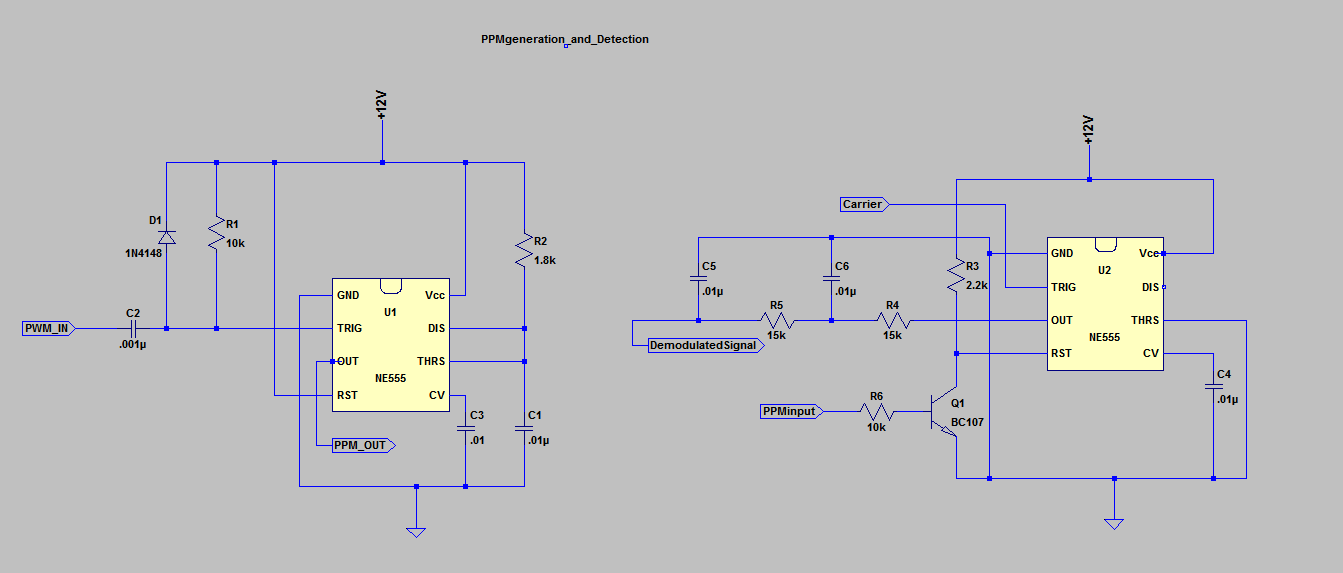
\includegraphics[height= 10cm]{ppmckt.png}
\caption{PPM generation and demodulation circuuit}
\label{ppmckt}
\end{sidewaysfigure}




%\section*{Components and Equipments Required}
%CRO (1), \\Signal generator(2),
%\\Resistors: $15\ k\Omega$(2), $10\ k\Omega$(1)
%\\Capacitors: $0.01\  \mu F$(2)
\section*{Procedure}
\begin{itemize}
\item
Connect the PWM generating circuit followed by PPM generating circuit  as shown in the diagram, Figure %\ref{pwmckt}.
\item
Feed the carrier pulse (square wave of $5 kHz$, $12V_{PP}$) from the function generator. 
\item
Feed the modulating message signal($500 Hz$, $\le 8 V_{pp}$) at pin-5 of PWM generator .
\item
Observe the outputof PWM and PPM on a CRO and plot the graphs of the input and output waveforms.
\item
Make the demodulating circuit as shown in the circuit diagram, Figure %\ref{pamckt}.
\item
Observe the input and output waveforms from PWM demodulation circuit. 
\end{itemize}
\section*{Observation}
Plot the graphs of input and output waveforms as observed on a CRO.
\section*{Result}

Implemented the PPM generation and demodulation circuits and plotted the waveforms.